

\documentclass{article} % version électronique
%\documentclass[titlepage,twoside,letterpaper,openright,12pt]{book} % version imprimée
%-----------------------------------------------------------------------------
% Entêtes et pieds 

%-----------------PDFLATEX----------------------
% Pour pdflatex, décommenter les lignes qui suivent
\usepackage[utf8]{inputenc} % encodage des caractères. choix: utf8, latin1, applemac
\usepackage[T1]{fontenc}
% choix du style de police (tout commenter pour les polices TeX habituelles [computer modern])
\usepackage{mathpazo} % utilise Palatino pour les mathématiques (mettre en premier)
\usepackage{tgpagella} % utilise la police TeX Gyre Pagella
%\usepackage{times} % utilise la police Times Roman

%-----------------XELATEX-----------------------
% Pour xelatex, décommenter plutôt les 6 lignes qui suivent:
%\XeTeXdefaultencoding utf-8
%\usepackage[no-math]{fontspec}
%\defaultfontfeatures{Mapping=tex-text} 
%\setmainfont[Ligatures={Rare}]{Didot}
%\setmonofont[Scale=0.9]{Lucida Sans Typewriter} 
%\setsansfont[Scale=0.9]{TeX Gyre Adventor} 
%-----------------------------------------------


\usepackage{amsfonts}		% ajoute des polices mathématique
\usepackage{amsmath}          % ajoute des environnements mathématiques
\usepackage{bm}				% ajoute des caractères grecs en gras
\usepackage{mathrsfs}		% ajoute une meilleure police calligraphique pour certains symboles
\usepackage{setspace} 		% gère l'interligne
% \usepackage[babel=true,kerning=french,protrusion=true,expansion=auto,spacing,tracking]{microtype}
\usepackage{graphicx}		% gère l'insertion des figures
\usepackage[export]{adjustbox}
\usepackage{ifpdf}
\usepackage{grffile}			% gère d'une façon saine d'esprit la reconnaissance automatique de format
\usepackage{subfig}			% permet d'ajouter des sous-figures
\usepackage{geometry}		% gère les dimensions du document (mise en page)
% \usepackage[x11names,svgnames]{xcolor}
\usepackage{url}            % permet de typographier des url
\usepackage{multirow}		% modifie la manière dont les descriptions de tableaux et figures sont disposées
\usepackage[format=hang,margin=5mm,font=small,labelfont=bf,labelsep=space]{caption}
\usepackage[section]{placeins}
\usepackage{epstopdf}
\usepackage[percent]{overpic}
\usepackage{verbatim}

\usepackage{tikz}
\usetikzlibrary{positioning}
\usetikzlibrary{backgrounds}
\usetikzlibrary{calc}
\usetikzlibrary{math}
\usetikzlibrary{external}
\tikzexternalize[prefix = tikzfigs/,mode=list and make,optimize command away=\includepdf] % activate!
%
\tikzset{
    % Defines a custom style which generates BOTH, .pdf and .png export
    svg export/.style={
        external/system call/.add={}%
        {; pdf2svg \image.pdf \image.svg}
    }
}
\tikzset{
    % Defines a custom style which generates BOTH, .pdf and .png export
    png export/.style={
        external/system call/.add={}%
        {; convert -density 300 -transparent white "\image.pdf" "\image.png"}
    }
}

\begin{document}
\tikzset{svg export} % Will be exported to a png as-well
Hello!
\centering

1
\begin{equation}
	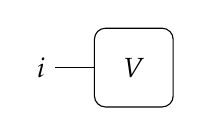
\begin{tikzpicture}[baseline=(current  bounding  box.center)]
		\node[fill = white, draw,rectangle,rounded corners,minimum width = 1.cm,minimum height = 1cm] at (0,0) (c) {$V$};
		\node[left = of c] at ++(0,0) (i) {$i$};
		\draw[-] (c) to (i);
	\end{tikzpicture}
\end{equation}

2
\begin{equation}
	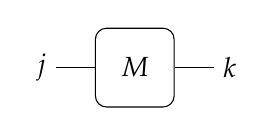
\begin{tikzpicture}[baseline=(current  bounding  box.center)]
		\node[fill = white, draw,rectangle,rounded corners,minimum width = 1.cm,minimum height = 1cm] at (0,0) (c) {$M$};
		\node[left = of c] at ++(0,0) (i) {$j$};
		\node[right = of c] at ++(0,0) (j) {$k$};
		\draw[-] (c) to (i);
		\draw[-] (c) to (j);
	\end{tikzpicture}
\end{equation}

3
\begin{equation}
	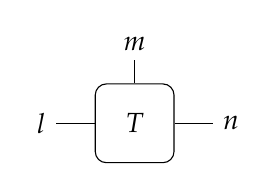
\begin{tikzpicture}[baseline=(current  bounding  box.center)]
		\node[fill = white, draw,rectangle,rounded corners,minimum width = 1cm,minimum height = 1cm] at (0,0) (c) {$T$};
		\node[left = of c] at ++(0,0) (i) {$l$};
		\node[above = of c] at ++(0,-0.2cm) (k) {$m$};
		\node[right = of c] at ++(0,0) (j) {$n$};
		\draw[-] (c) to (i);
		\draw[-] (c) to (j);
		\draw[-] (c) to (k);
	\end{tikzpicture}
\end{equation}

4
\begin{equation}
	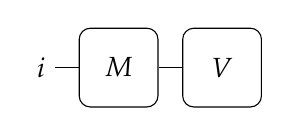
\begin{tikzpicture}[baseline=(current  bounding  box.center)]
		\node[fill = white, draw,rectangle,rounded corners,minimum width = 1cm,minimum height = 1cm] at (0,0) (v) {$V$};
		\node[left = 0.3cm of v, fill = white, draw,rectangle,rounded corners,minimum width = 1cm,minimum height = 1cm] (m) {$M$};
		\node[left = 0.3cm of m]  (i) {$i$};
		\draw[-] (m) to (i);
		\draw[-] (m) to (v);
	\end{tikzpicture}
\end{equation}

5
\begin{equation}
	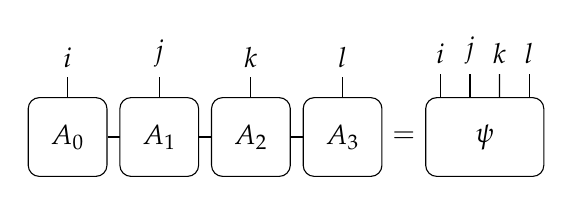
\begin{tikzpicture}[baseline=(current  bounding  box.center)]
		\node[fill = white, draw,rectangle,rounded corners,minimum width = 1.5cm,minimum height = 1cm] at (0,0) (c) {$\psi$};
		\node[left = 0cm of c] (eq) {$=$};
		\node[left = 0cm of eq,fill = white, draw,rectangle,rounded corners,minimum width = 1cm,minimum height = 1cm] (a3)
		{$
				A_3
			$};
		\node[left = .15cm of a3,fill = white, draw,rectangle,rounded corners,minimum width = 1cm,minimum height = 1cm] (a2)
		{$
				A_2
			$};
		\node[left = 0.15cm of a2,fill = white, draw,rectangle,rounded corners,minimum width = 1cm,minimum height = 1cm] (a1)
		{$
				A_1
			$};
		\node[left = 0.15cm of a1,fill = white, draw,rectangle,rounded corners,minimum width = 1cm,minimum height = 1cm] (a0)
		{$
				A_0
			$};
		\node[ above = 0.25cm of a0 ] (ia) {$i$};
		\node[ above = 0.25cm of a1 ] (ja) {$j$};
		\node[ above = 0.25cm of a2 ]  (ka) {$k$};
		\node[ above = 0.25cm of a3 ]  (la) {$l$};
		\node[ above = of c ] at ++(-0.5625,-0.2) (i) {$i$};
		\node[ above = of c ] at ++(-0.1875,-0.2) (j) {$j$};
		\node[ above = of c ] at ++(0.18755,-0.2) (k) {$k$};
		\node[ above = of c ] at ++(0.5625,-0.2) (l) {$l$};
		\begin{scope}[on background layer]
			\draw[black,-] (a0) to (a3);
			\draw[black,-] (a0) to (ia);
			\draw[black,-] (a1) to (ja);
			\draw[black,-] (a2) to (ka);
			\draw[black,-] (a3) to (la);
			\draw[below = of c,black,-] ++(-0.5625,0) to (i);
			\draw[below = of c,black,-] ++(-0.1875,0) to (j);
			\draw[below = of c,black,-] ++(0.1875,0) to (k);
			\draw[below = of c,black,-] ++(0.5625,0) to (l);
		\end{scope}
	\end{tikzpicture}
	\label{eq:tenspsi_plein}
\end{equation}

6
\begin{equation}
	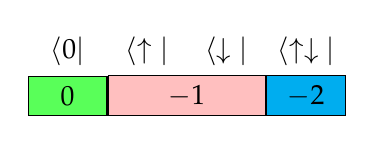
\begin{tikzpicture}[baseline=(current  bounding  box.center)]
		\node[fill = pink, draw,rectangle,minimum width = 2cm,minimum height = 0.5cm] at (0,0) (v1) {$-1$};
		\node[left = 0cm of v1,fill = green!65, draw,rectangle,minimum width = 1cm,minimum height = 0.5cm] (v0) {$0$};
		\node[right = 0cm of v1,fill = cyan, draw,rectangle,minimum width = 1cm,minimum height = 0.5cm] (v2) {$-2$};
		\node[above = 0cm of v0] (s0) {$\langle 0|$};
		\node[above = 0cm of v2] (supdn) {$\langle \uparrow \downarrow |$};
		\node at ($(s0)!0.333!(supdn)$) (sup) {$ \langle \uparrow |$};
		\node at ($ (s0)!0.666!(supdn) $) (sdn) {$ \langle \downarrow |$};
	\end{tikzpicture}
\end{equation}

7
\begin{equation}
	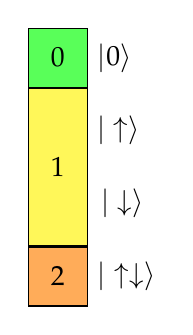
\begin{tikzpicture}[baseline=(current  bounding  box.center)]
		\node[fill = yellow!65, draw,rectangle,minimum width = 0.75cm,minimum height = 2cm] at (0,0) (v1) {$1$};
		\node[above = 0cm of v1,fill = green!65, draw,rectangle,minimum width = 0.75cm,minimum height = 0.75cm] (v0) {$0$};
		\node[below = 0cm of v1,fill = orange!65, draw,rectangle,minimum width = .75cm,minimum height = 0.75cm] (v2) {$2$};
		\node[right = 0cm of v0] (s0) {$| 0 \rangle$};
		\node[right = 0cm of v2] (supdn) {$| \uparrow \downarrow \rangle$};
		\node at ($(s0)!0.333!(supdn)$) (sup) {$ | \uparrow \rangle$};
		\node at ($ (s0)!0.666!(supdn) $) (sdn) {$ | \downarrow \rangle $};
	\end{tikzpicture}
\end{equation}

8
\begin{equation}
	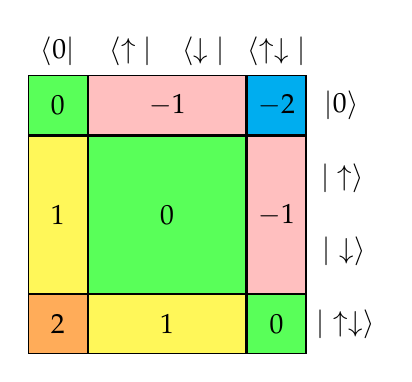
\begin{tikzpicture}[baseline=(current  bounding  box.center)]
		\node[fill = pink, draw,rectangle,minimum width = 2cm,minimum height = 0.75cm] at (0,0) (v1) {$-1$};
		\node[left = 0cm of v1,fill = green!65, draw,rectangle,minimum width = 0.75cm, minimum height = 0.75cm] (v0) {$0$};
		\node[right = 0cm of v1,fill = cyan, draw,rectangle,minimum width = 0.75 cm, minimum height = 0.75cm] (v2) {$-2$};
		\node[below = 0cm of v1, fill =  green!65, draw,rectangle,minimum width = 2cm,minimum height = 2cm] (v1m1) {$0$};
		\node[left = 0cm of v1m1,fill = yellow!65, draw,rectangle,minimum width = 0.75cm, minimum height = 2cm] (v0m1) {$1$};
		\node[below = 0cm of v1m1,fill = yellow!65, draw,rectangle,minimum width = 2cm, minimum height = 0.75cm] (v1m2) {$1$};
		\node[right = 0cm of v1m1, fill = pink, draw,rectangle,minimum width = 0.75cm,minimum height = 2cm]  (v2m1) {$-1$};
		\node[below = 0cm of v2m1, fill =  green!65, draw,rectangle,minimum width = .75cm,minimum height = .75cm] (v2m2) {$0$};
		\node[below = 0cm of v0m1,fill = orange!65, draw,rectangle,minimum width = 0.75cm, minimum height = .75cm] (v0m2) {$2$};à
		\node[above = 0cm of v0] (s0) {$\langle 0|$};
		\node[above = 0cm of v2] (supdn) {$\langle \uparrow \downarrow |$};
		\node at ($(s0)!0.333!(supdn)$) (sup) {$ \langle \uparrow |$};
		\node at ($ (s0)!0.666!(supdn) $) (sdn) {$ \langle \downarrow |$};
		\node[right = 0.1cm of v2] (ss0) {$|0\rangle$};
		\node[right = 0cm of v2m2] (ssupdn) {$|\uparrow \downarrow \rangle$};
		\node at ($(ss0)!0.333!(ssupdn)$) (ssup) {$|\uparrow \rangle$};
		\node at ($ (ss0)!0.666!(ssupdn) $) (ssdn) {$|\downarrow \rangle$};
	\end{tikzpicture}
\end{equation}

9
\begin{equation}
	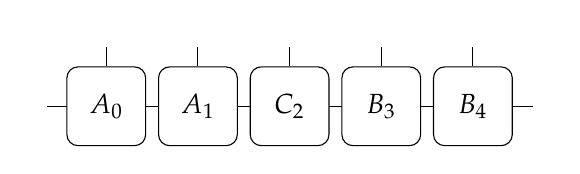
\begin{tikzpicture}[baseline=(current  bounding  box.center)]
		\node[fill = white, draw,rectangle,rounded corners,minimum width = 1cm,minimum height = 1cm] at (0,0) (a3)
		{$
				B_4
			$};
		\node[left = .15cm of a3,fill = white, draw,rectangle,rounded corners,minimum width = 1cm,minimum height = 1cm] (a2)
		{$
				B_3
			$};
		\node[left = .15cm of a2,fill = white, draw,rectangle,rounded corners,minimum width = 1cm,minimum height = 1cm] (c)
		{$
				C_2
			$};
		\node[left = 0.15cm of c,fill = white, draw,rectangle,rounded corners,minimum width = 1cm,minimum height = 1cm] (a1)
		{$
				A_1
			$};
		\node[left = 0.15cm of a1,fill = white, draw,rectangle,rounded corners,minimum width = 1cm,minimum height = 1cm] (a0)
		{$
				A_0
			$};
		\node[ above = 0.25cm of a0 ] (ia) {};
		\node[ above = 0.25cm of a1 ] (ja) {};
		\node[ above = 0.25cm of a2 ]  (ka) {};
		\node[ above = 0.25cm of a3 ]  (la) {};
		\node[ above = 0.25cm of c ]  (ma) {};
		\node[ left = 0.25cm of a0 ]  (ga) {};
		\node[ right = 0.25cm of a3 ]  (da) {};

		\begin{scope}[on background layer]
			\draw[black,-] (da) to (ga);
			\draw[black,-] (a0) to (ia);
			\draw[black,-] (a1) to (ja);
			\draw[black,-] (a2) to (ka);
			\draw[black,-] (a3) to (la);
			\draw[black,-] (c) to (ma);

		\end{scope}
	\end{tikzpicture}
\end{equation}

10
\begin{equation}
	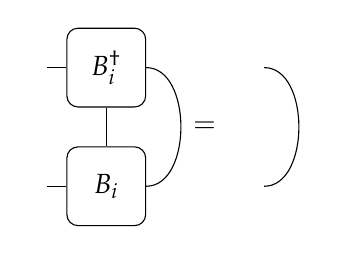
\begin{tikzpicture}[baseline=(current  bounding  box.center)]
		\node[fill = white, draw,rectangle,rounded corners,minimum width = 1cm,minimum height = 1cm] at (0,0) (b)
		{$
				B_i
			$};

		\node[above = of b, fill = white, draw,rectangle,rounded corners,minimum width = 1cm,minimum height = 1cm] at (0,0) (bd)
		{$
				B^\dagger_i
			$};

		\node[left = 0.25cm of bd]  (bda) {};
		\node[left = 0.25cm of b]  (ba) {};

		\node at ($ (b)!0.5!(bd) + (1.25cm,0) $) (eq) {$=$};

		\node[right = 1.25cm of bd] (id) {};
		\node[right = 1.25cm of b] (iid) {};

		\begin{scope}[on background layer]
			\draw[black,-] (b) to[out=0,in=0] (bd);
			\draw[black,-] (bd) to (b);
			\draw[black,-] (bd) to (bda);
			\draw[black,-] (b) to (ba);
			\draw[black,-] (id) to[out=0,in=0] (iid);

		\end{scope}
	\end{tikzpicture}
\end{equation}

11
\begin{equation}
	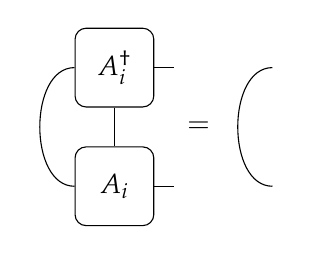
\begin{tikzpicture}[baseline=(current  bounding  box.center)]
		\node[fill = white, draw,rectangle,rounded corners,minimum width = 1cm,minimum height = 1cm] at (0,0) (b)
		{$
				A_i
			$};

		\node[above = of b, fill = white, draw,rectangle,rounded corners,minimum width = 1cm,minimum height = 1cm] at (0,0) (bd)
		{$
				A^\dagger_i
			$};

		\node[right = 0.25cm of bd]  (bda) {};
		\node[right = 0.25cm of b]  (ba) {};

		\node at ($ (b)!0.5!(bd) + (1.07cm,0) $) (eq) {$=$};

		\node[right = 1.5cm of bd] (id) {};
		\node[right = 1.5cm of b] (iid) {};

		\begin{scope}[on background layer]
			\draw[black,-] (b) to[out=180,in=180] (bd);
			\draw[black,-] (bd) to (b);
			\draw[black,-] (bd) to (bda);
			\draw[black,-] (b) to (ba);
			\draw[black,-] (id) to[out=180,in=180] (iid);

		\end{scope}
	\end{tikzpicture}
\end{equation}

11
\begin{equation}
	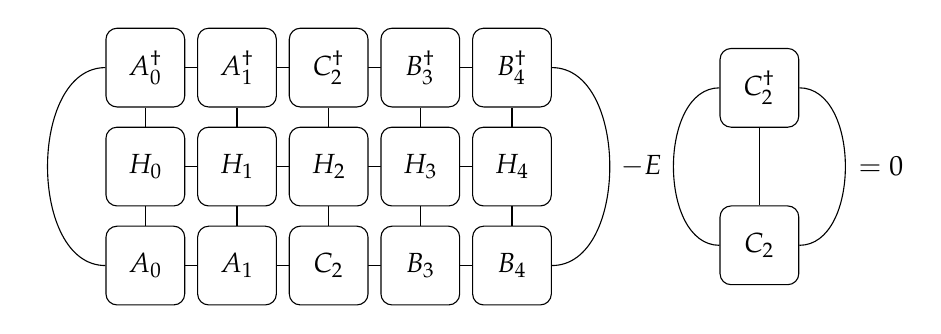
\begin{tikzpicture}[baseline=(current  bounding  box.center)]
		\node[fill = white, draw,rectangle,rounded corners,minimum width = 1cm,minimum height = 1cm] at (0,0) (a3) {$B_4$};
		\node[left = .15cm of a3,fill = white, draw,rectangle,rounded corners,minimum width = 1cm,minimum height = 1cm] (a2)
		{$ B_3$};
		\node[left = .15cm of a2,fill = white, draw,rectangle,rounded corners,minimum width = 1cm,minimum height = 1cm] (c)
		{$C_2$};
		\node[left = 0.15cm of c,fill = white, draw,rectangle,rounded corners,minimum width = 1cm,minimum height = 1cm] (a1)
		{$A_1$};
		\node[left = 0.15cm of a1,fill = white, draw,rectangle,rounded corners,minimum width = 1cm,minimum height = 1cm] (a0)
		{$A_0$};
		
		\node[above = 1.5cm of a3, fill = white, draw,rectangle,rounded corners,minimum width = 1cm,minimum height = 1cm] (ad3)
		{$B^\dagger_4$};
		\node[left = .15cm of ad3,fill = white, draw,rectangle,rounded corners,minimum width = 1cm,minimum height = 1cm] (ad2)
		{$B^\dagger_3$};
		\node[left = .15cm of ad2,fill = white, draw,rectangle,rounded corners,minimum width = 1cm,minimum height = 1cm] (cd)
		{$C^\dagger_2$};
		\node[left = 0.15cm of cd,fill = white, draw,rectangle,rounded corners,minimum width = 1cm,minimum height = 1cm] (ad1)
		{$A^\dagger_1$};
		\node[left = 0.15cm of ad1,fill = white, draw,rectangle,rounded corners,minimum width = 1cm,minimum height = 1cm] (ad0)
		{$A^\dagger_0$};
		
		\node[fill = white, draw,rectangle,rounded corners,minimum width = 1cm,minimum height = 1cm] at ($ (ad3)!0.5!(a3) $) (h4)
		{$H_4$};
		\node[left = .15cm of h4,fill = white, draw,rectangle,rounded corners,minimum width = 1cm,minimum height = 1cm] (h3)
		{$H_3$};
		\node[left = .15cm of h3,fill = white, draw,rectangle,rounded corners,minimum width = 1cm,minimum height = 1cm] (h2)
		{$H_2$};
		\node[left = 0.15cm of h2,fill = white, draw,rectangle,rounded corners,minimum width = 1cm,minimum height = 1cm] (h1)
		{$H_1$};
		\node[left = 0.15cm of h1,fill = white, draw,rectangle,rounded corners,minimum width = 1cm,minimum height = 1cm] (h0)
		{$H_0$};

		\node[ right = .75cm of h4 ]  (ga) {$- E $};

		\node[fill = white, draw,rectangle,rounded corners,minimum width = 1cm,minimum height = 1cm] 
		at ($ (ga)+(1.5cm,1.cm) $) (cb) {$C^\dagger_2$};
		\node[fill = white, draw,rectangle,rounded corners,minimum width = 1cm,minimum height = 1cm] 
		at ($ (ga)+(1.5cm,-1.cm) $) (cdb) {$C_2$};
		\node[ right = 2.25cm of ga ]  (ha) {$ = 0 $};

		\begin{scope}[on background layer]
			\draw[black,-] (a0) to (ad0);
			\draw[black,-] (a1) to (ad1);
			\draw[black,-] (a2) to (ad2);
			\draw[black,-] (a3) to (ad3);
			\draw[black,-] (a0) to (a3);
			\draw[black,-] (ad0) to (ad3);
			\draw[black,-] (c) to (cd);
			\draw[black,-] (h0) to (h4);
			\draw[black,-] (a0) to[out=180, in=180] (ad0);
			\draw[black,-] (a3) to[out=0, in=0] (ad3);
			\draw[black,-] (cb) to[out=0, in=0] (cdb);
			\draw[black,-] (cb) to[out=180, in=180] (cdb);
			\draw[black,-] (cb) to (cdb);
		\end{scope}
	\end{tikzpicture}
\end{equation}
Who are you?

\pagebreak

Bye!

\end{document}